\section{Blah blah}

Three papers: \cite{Lloyd:Time}, \cite{Marletto:Evolution}, \cite{Prvanovic}.

And an experiment: \cite{Moreva:synthetic,Moreva:illustration}.

The basic idea is an additional Hilbert space $\mathcal{H}_T$ where time is an observable
corresponding to
a self-adjoint operator whose mathematical properties are the same of position in the
ordinary Hilbert space of a quantum particle in one dimension.

In this language, the ordinary Hilbert space can be labeled $\mathcal{H}_S$;
and we consider the product space $\mathcal{H}_T \otimes \mathcal{H}_S$ as
the space in which both time and position are observables, and they act as
$\hat{t} \otimes \idop_S$ and $\idop_T \otimes \hat{x}$
respectively.

\section{Questions and observations on Lloyd's paper}

With regards to \cite{Lloyd:Time}, section B, \textit{Measurement}.

\begin{enumerate}
  \item What is a memory system in quantum mechanics? 
  \begin{itemize}
    \item Do they mean a non-Markovian system? Look at \cite{MeasurementMarkovian}\dots
    \item Memory in the sense of the Maxwell daemon?
    \item
      Any general theory of quantum memory systems? Fiducial states?
      Yes, see \ref{sec:qmemory} or most importantly \cite[Ch.~3]{PreskillMeasurement}.
    \item memory kernels \cite{CarmichaelOQS2017}
  \end{itemize}
  \item ``\emph{the case where a measurement is performed at time t1}'' suggests they are back to time as an external parameter\dots
\end{enumerate}

\section{Memory systems (and fiducial state?)}\label{sec:qmemory}
Besides, and perhaps better than the below, see \cite[Ch.~3]{PreskillMeasurement},
which cover and expands topics discussed in \cite{open_systems}.

\clearpage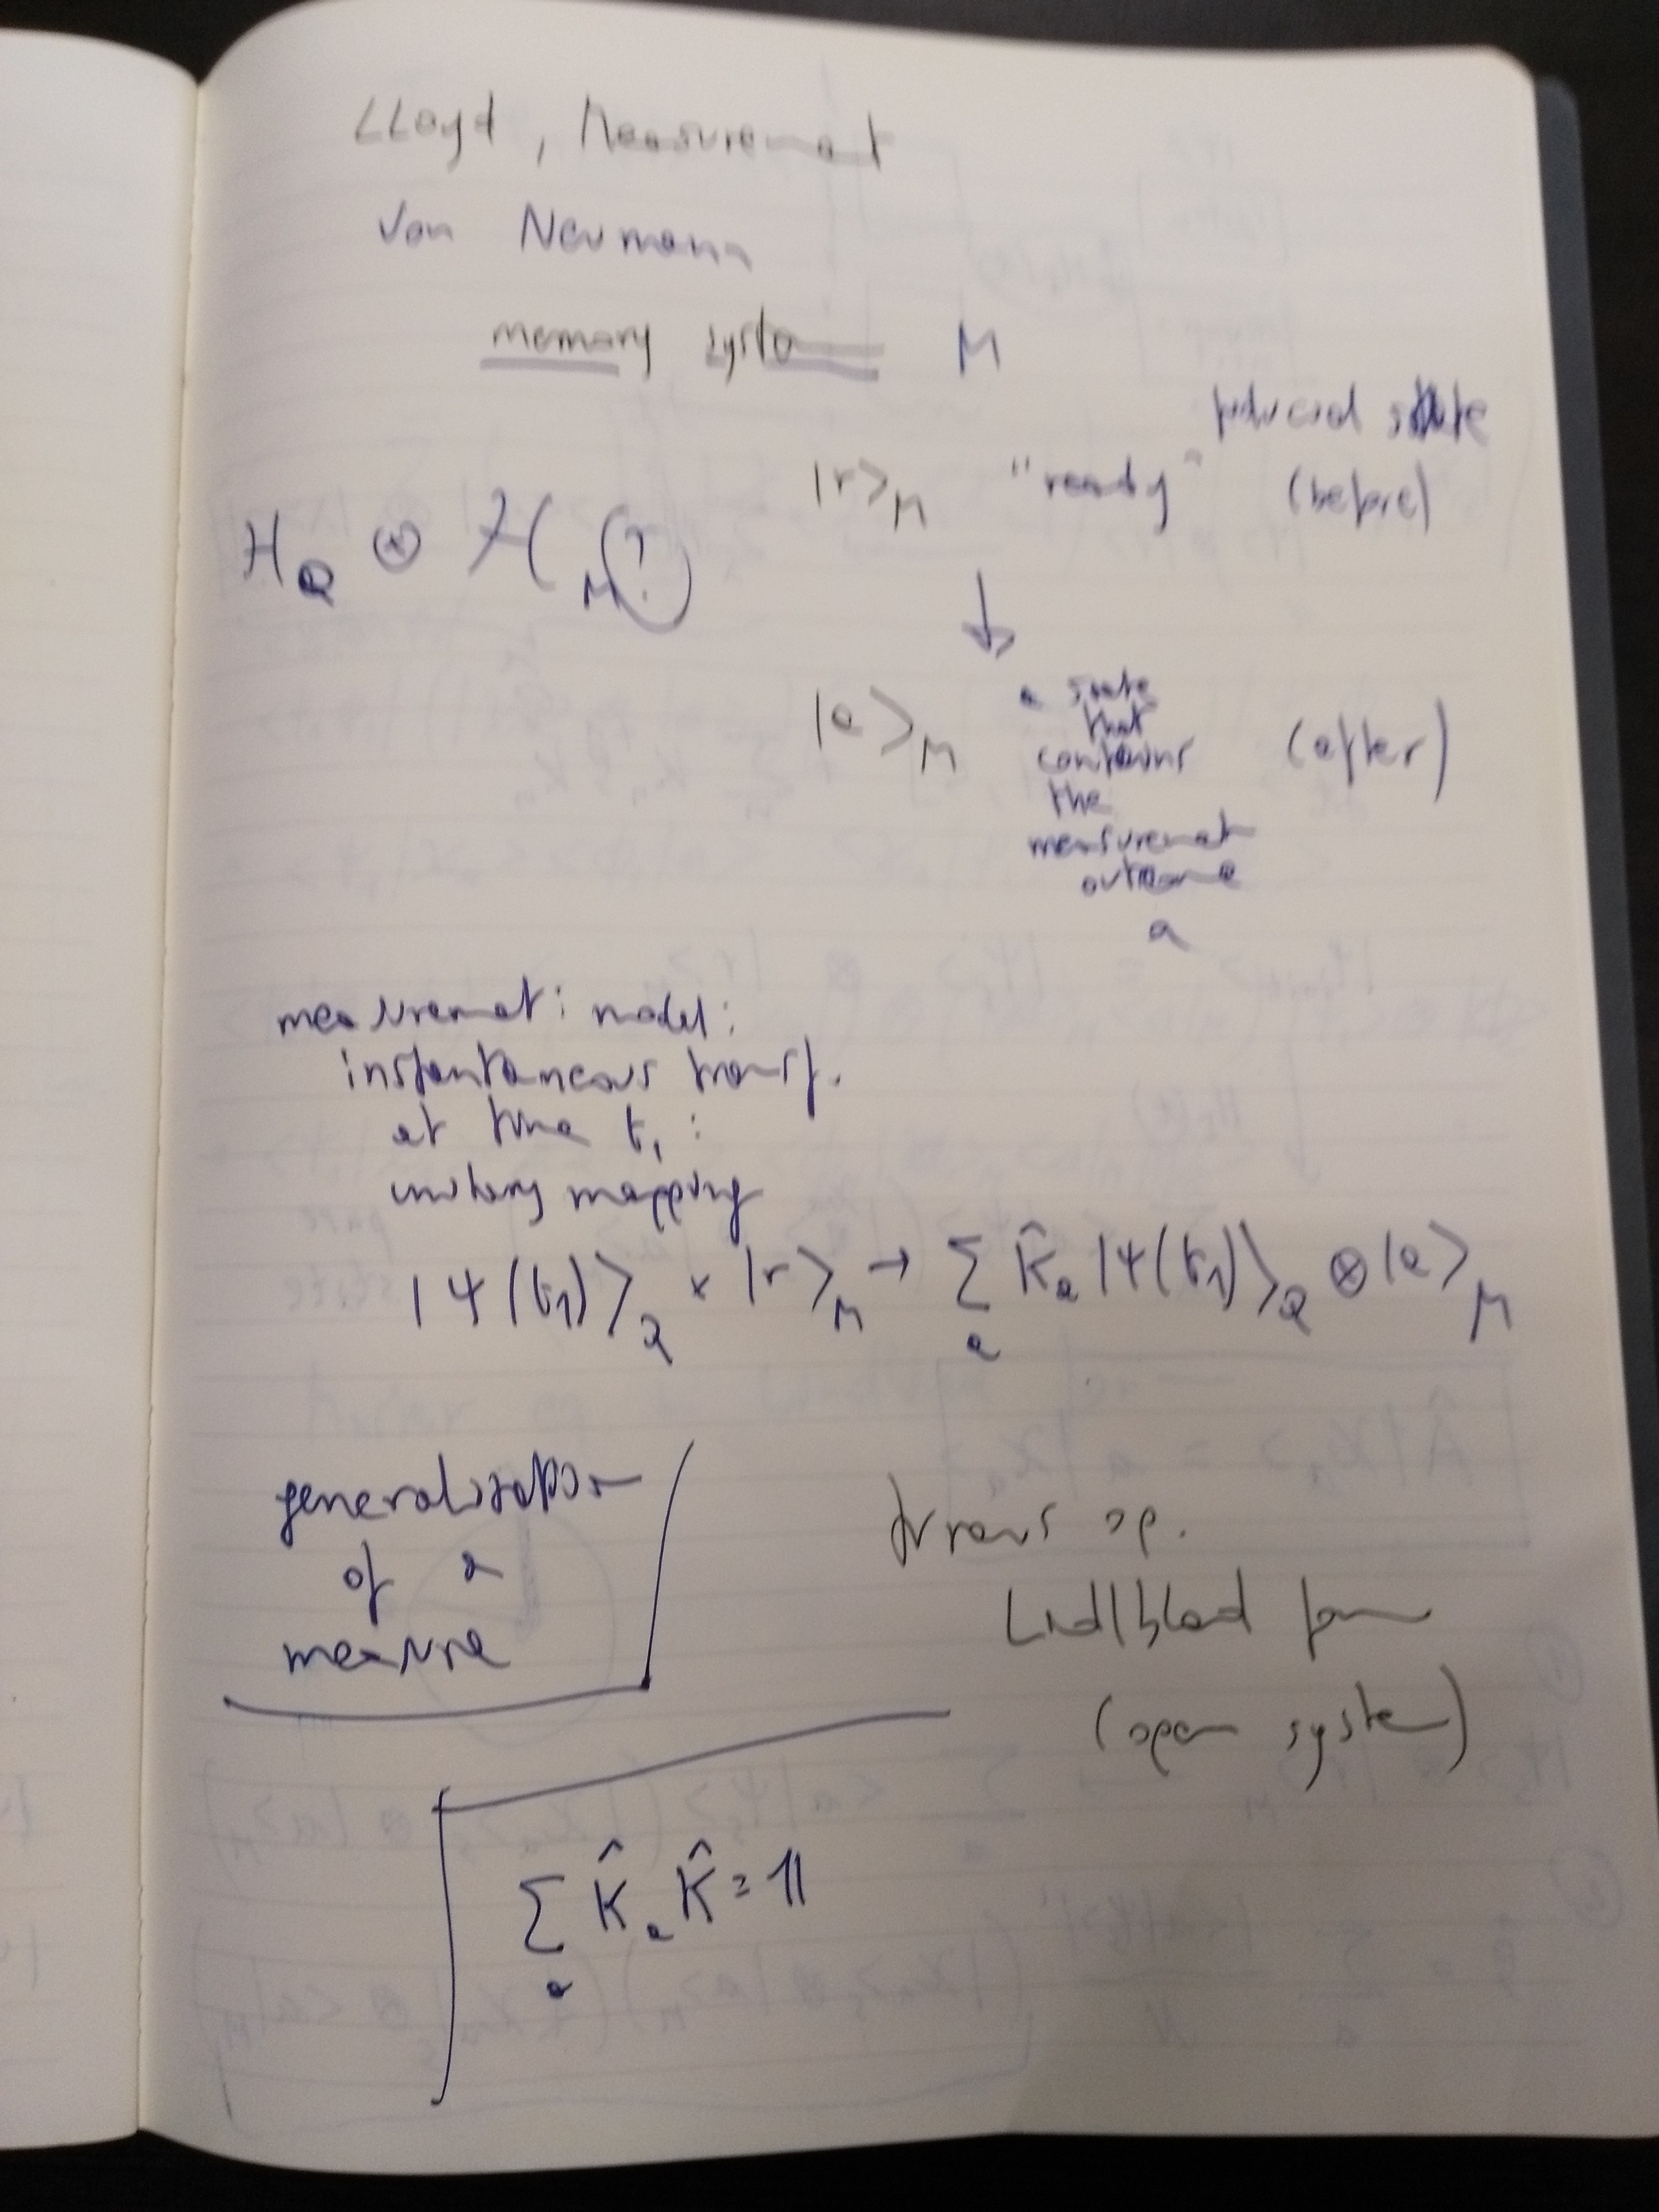
\includegraphics[width=\linewidth]{img/pw/qmem/1.jpg}
\clearpage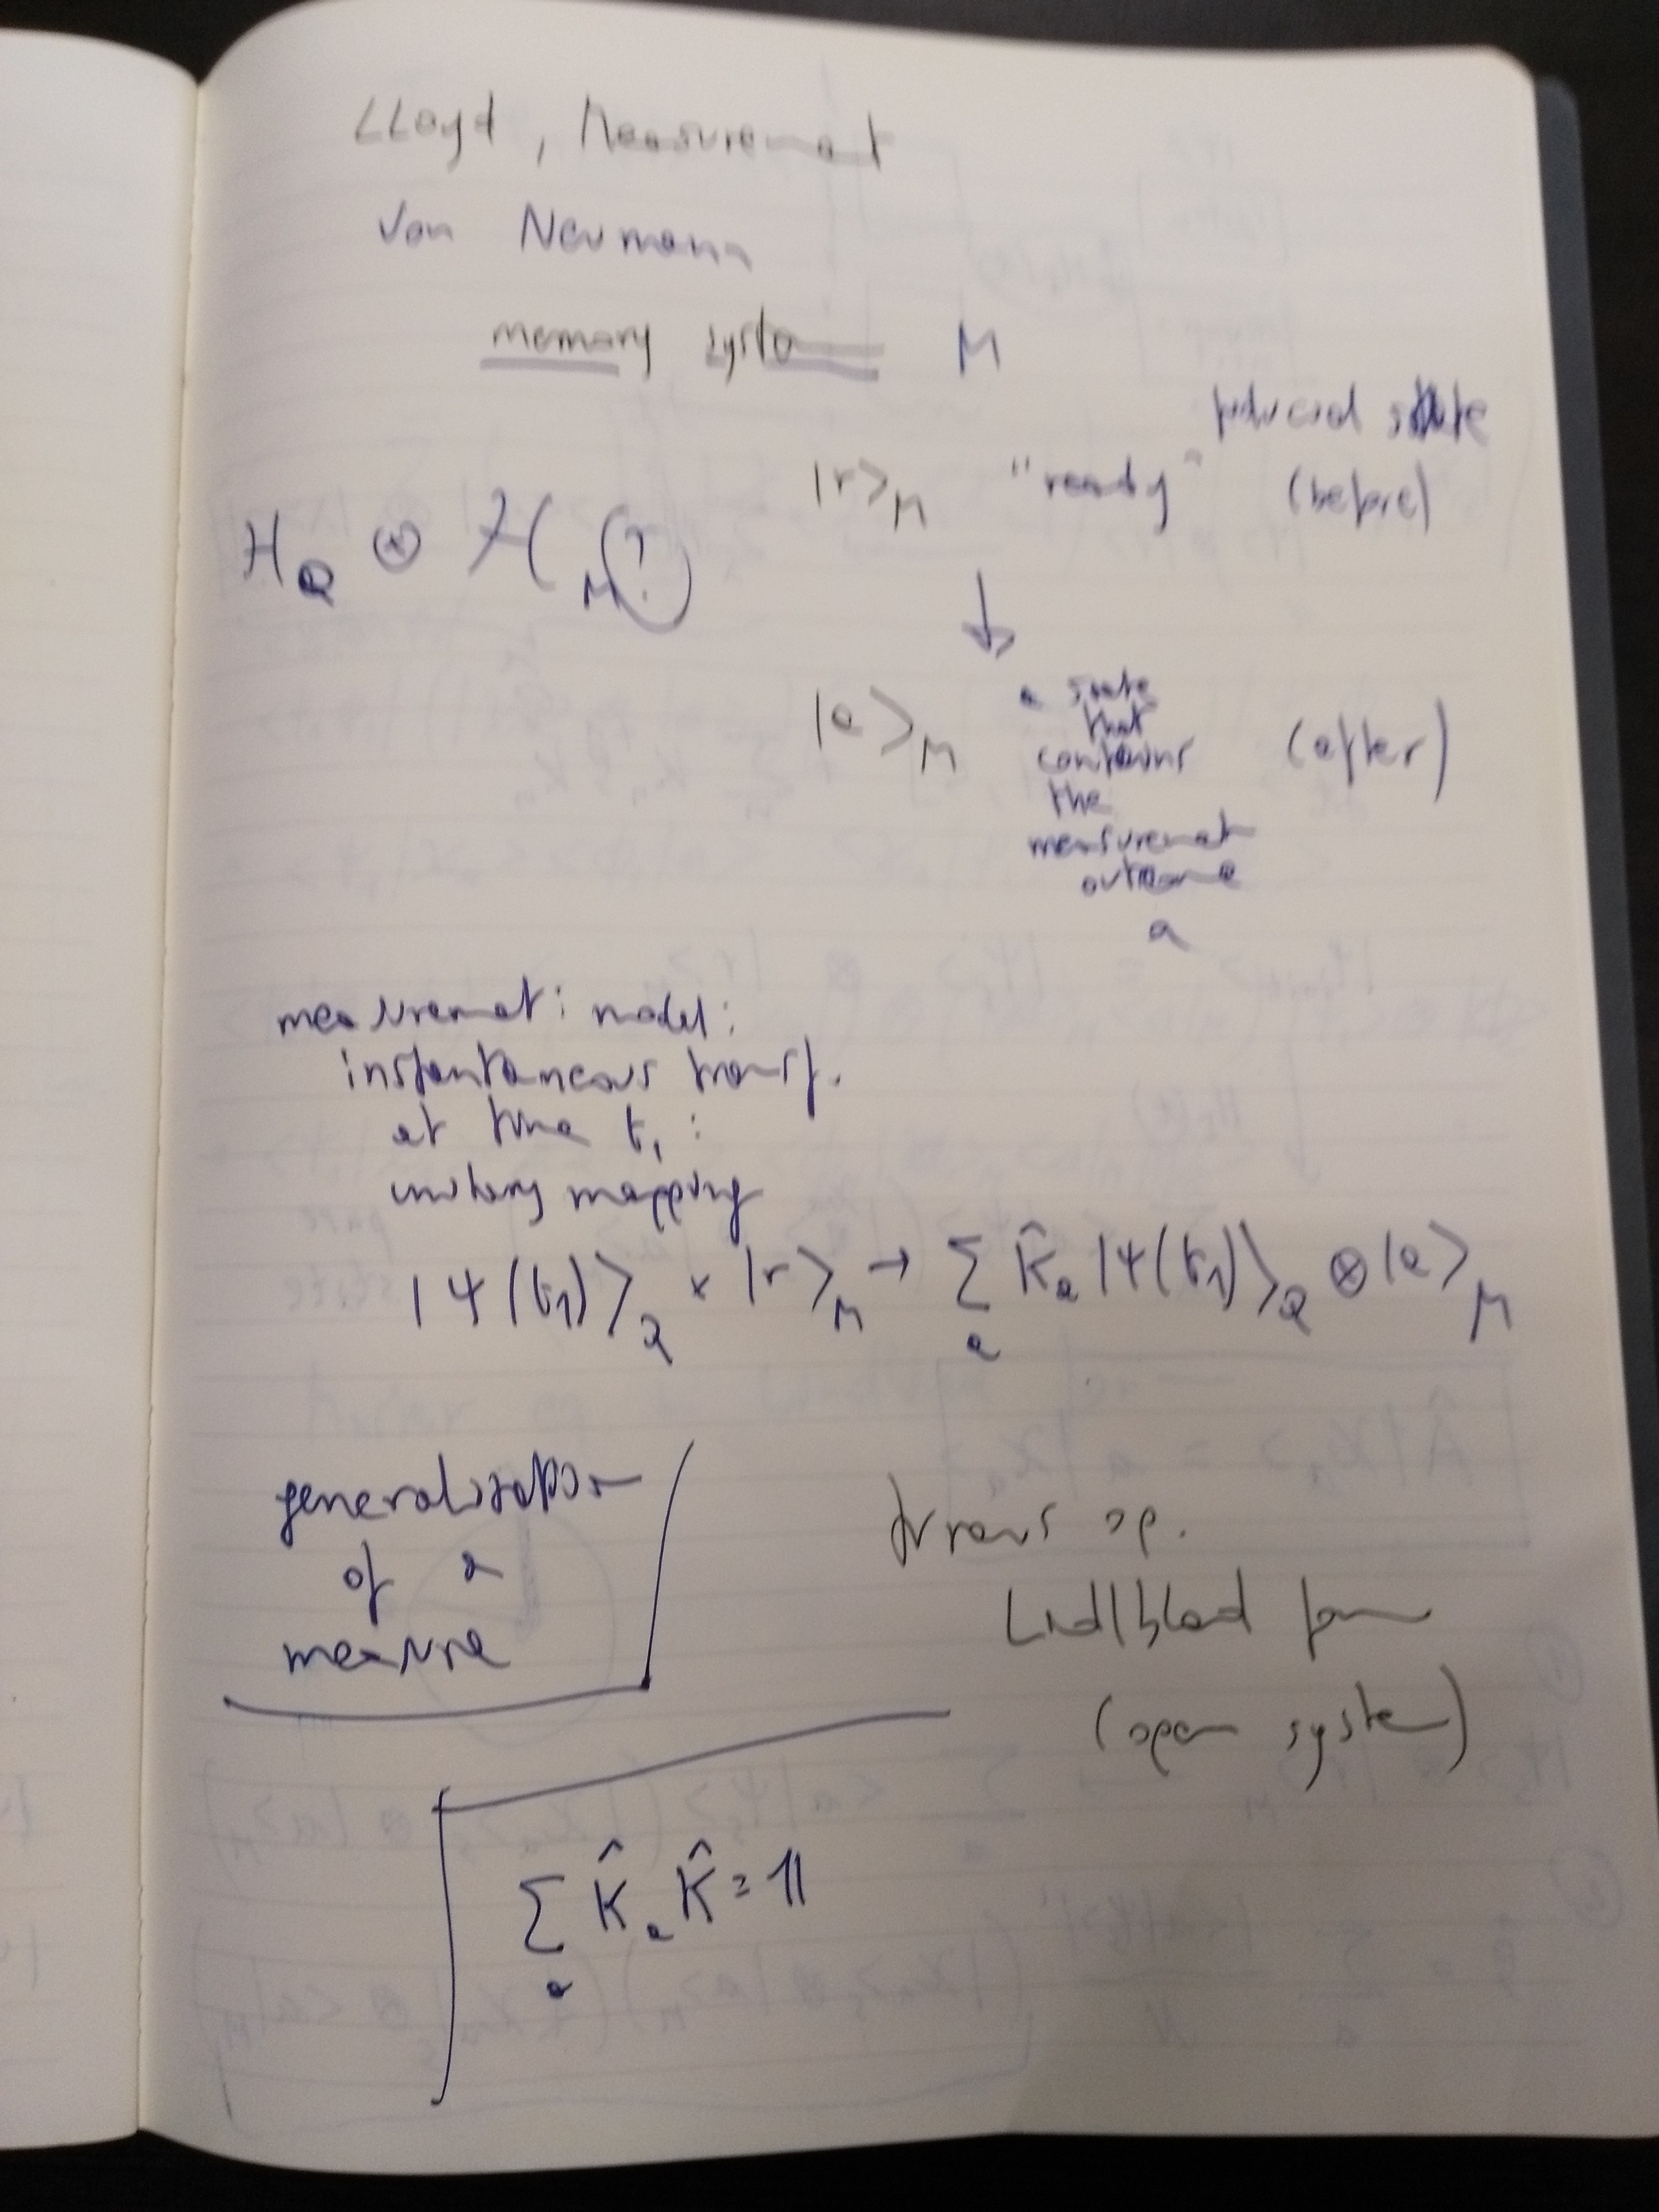
\includegraphics[width=\linewidth]{img/pw/qmem/2.jpg}
\clearpage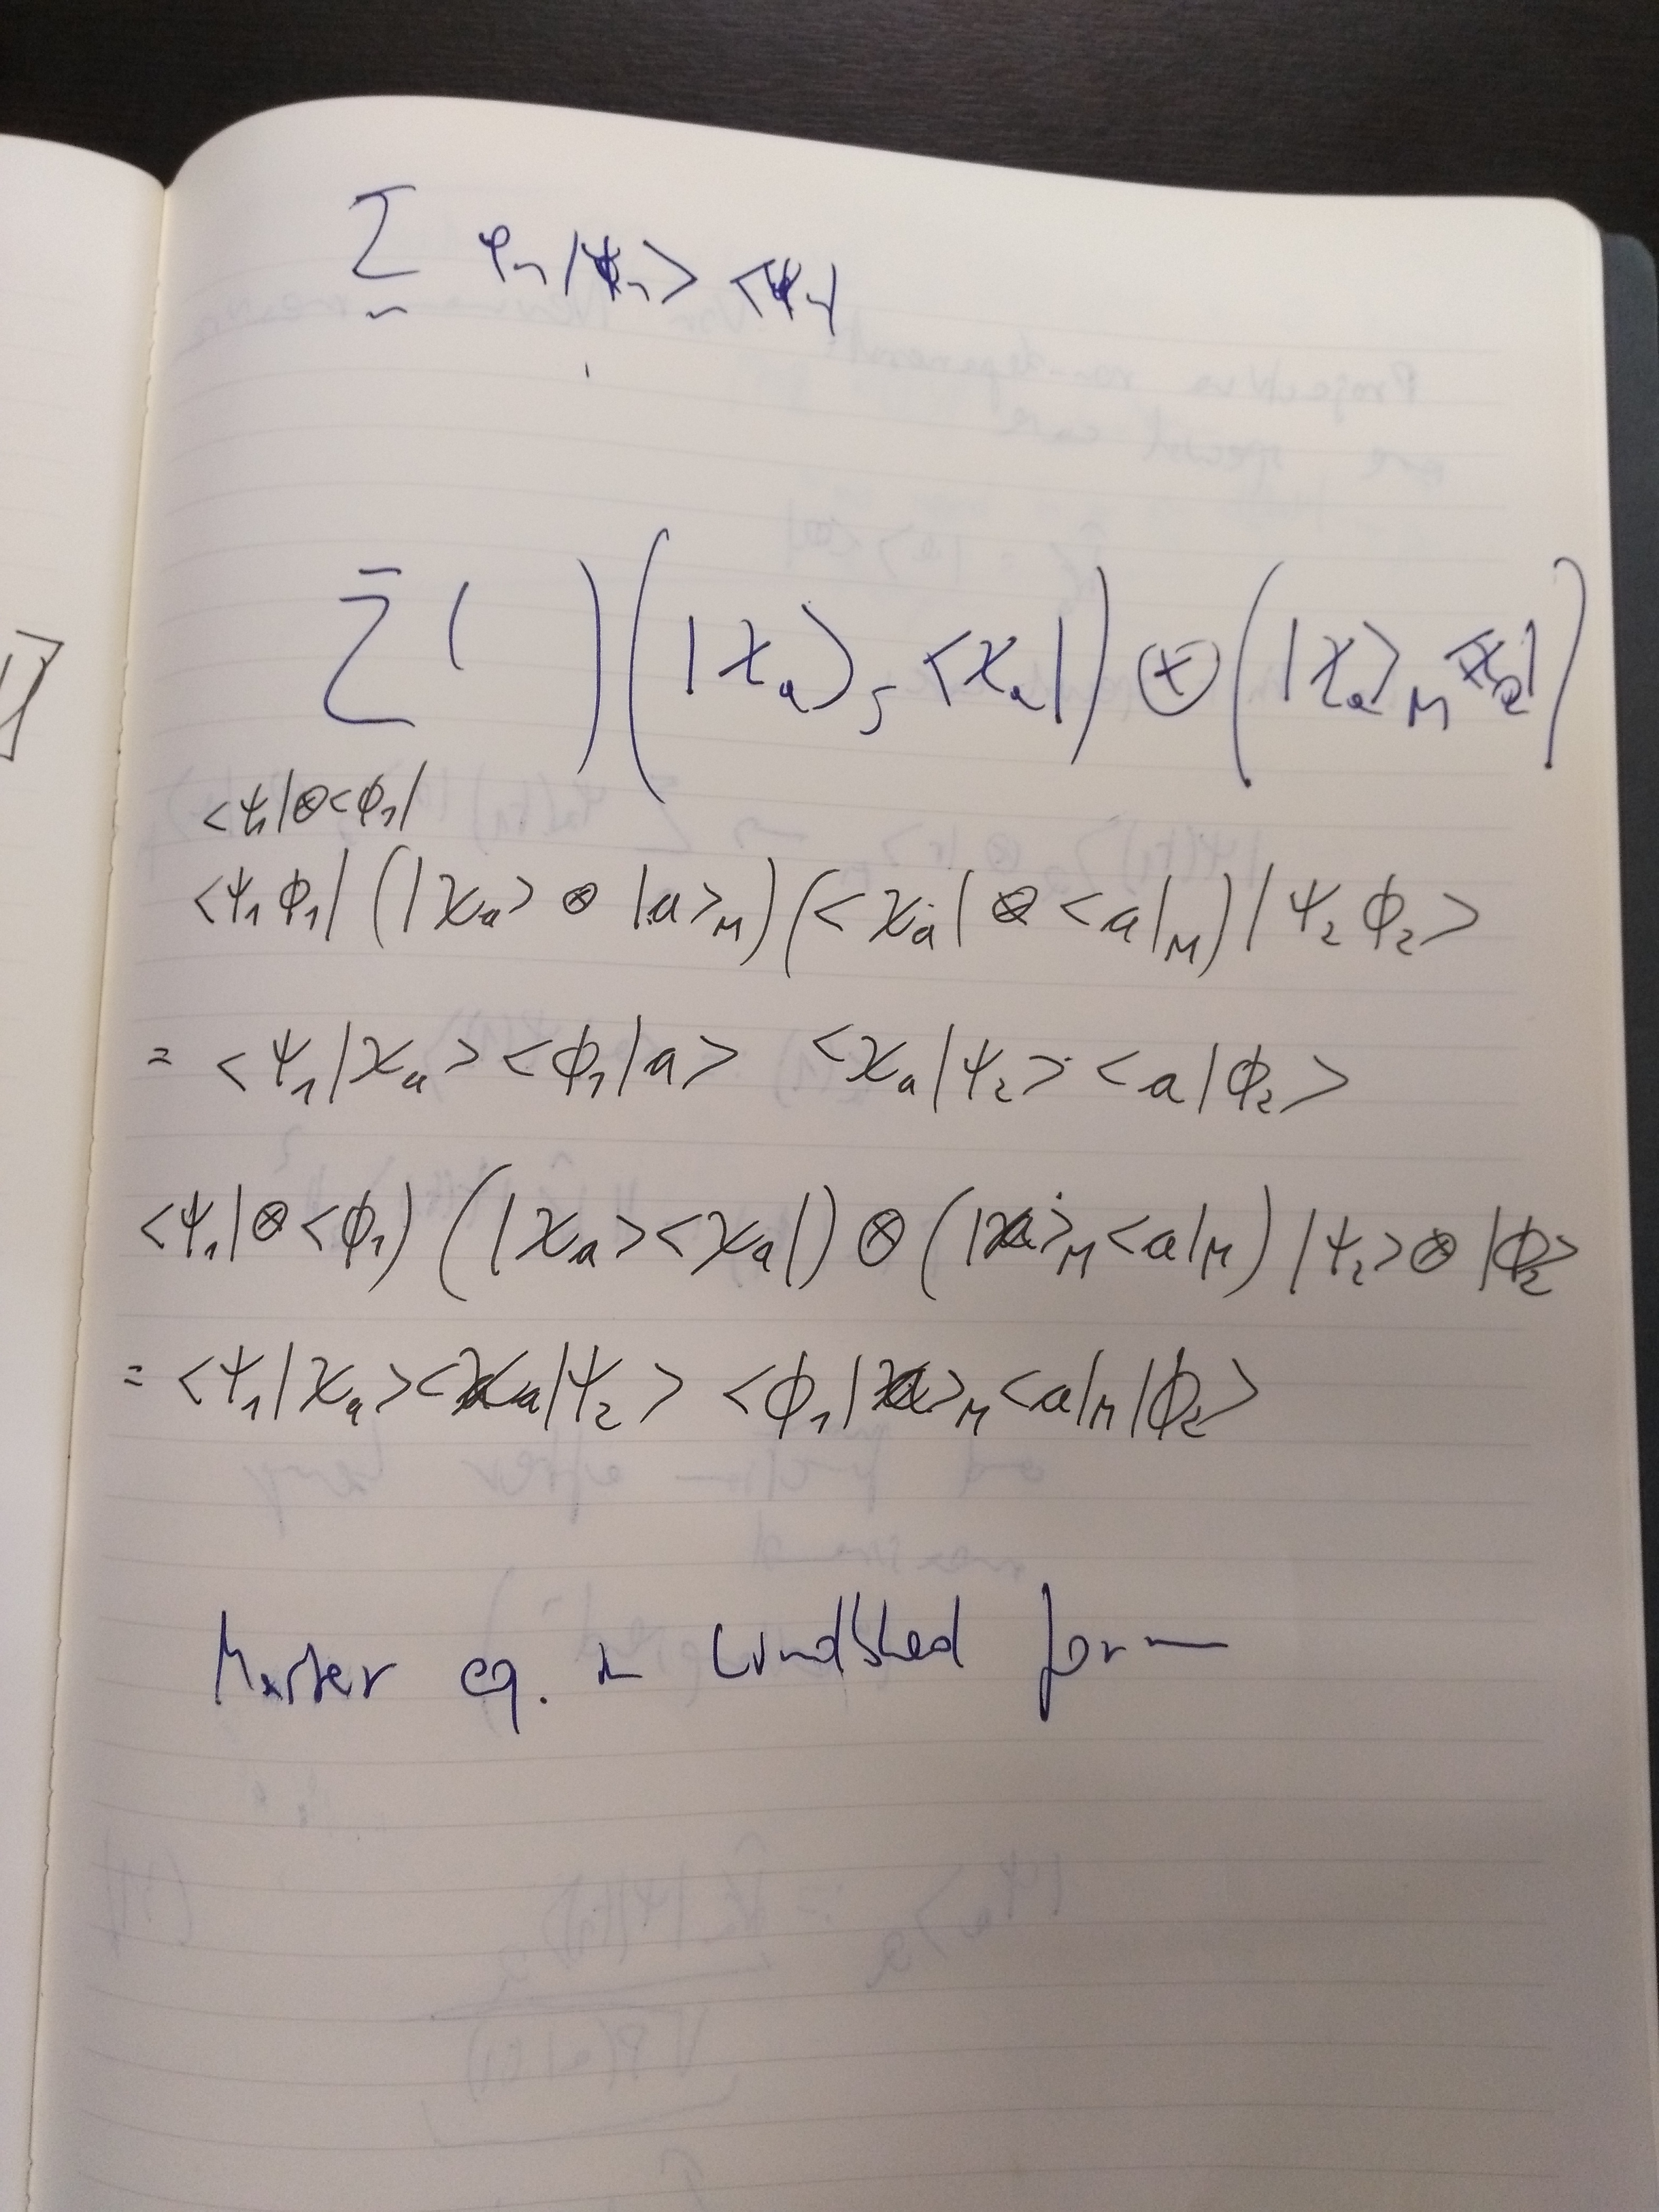
\includegraphics[width=\linewidth]{img/pw/qmem/3.jpg}
\clearpage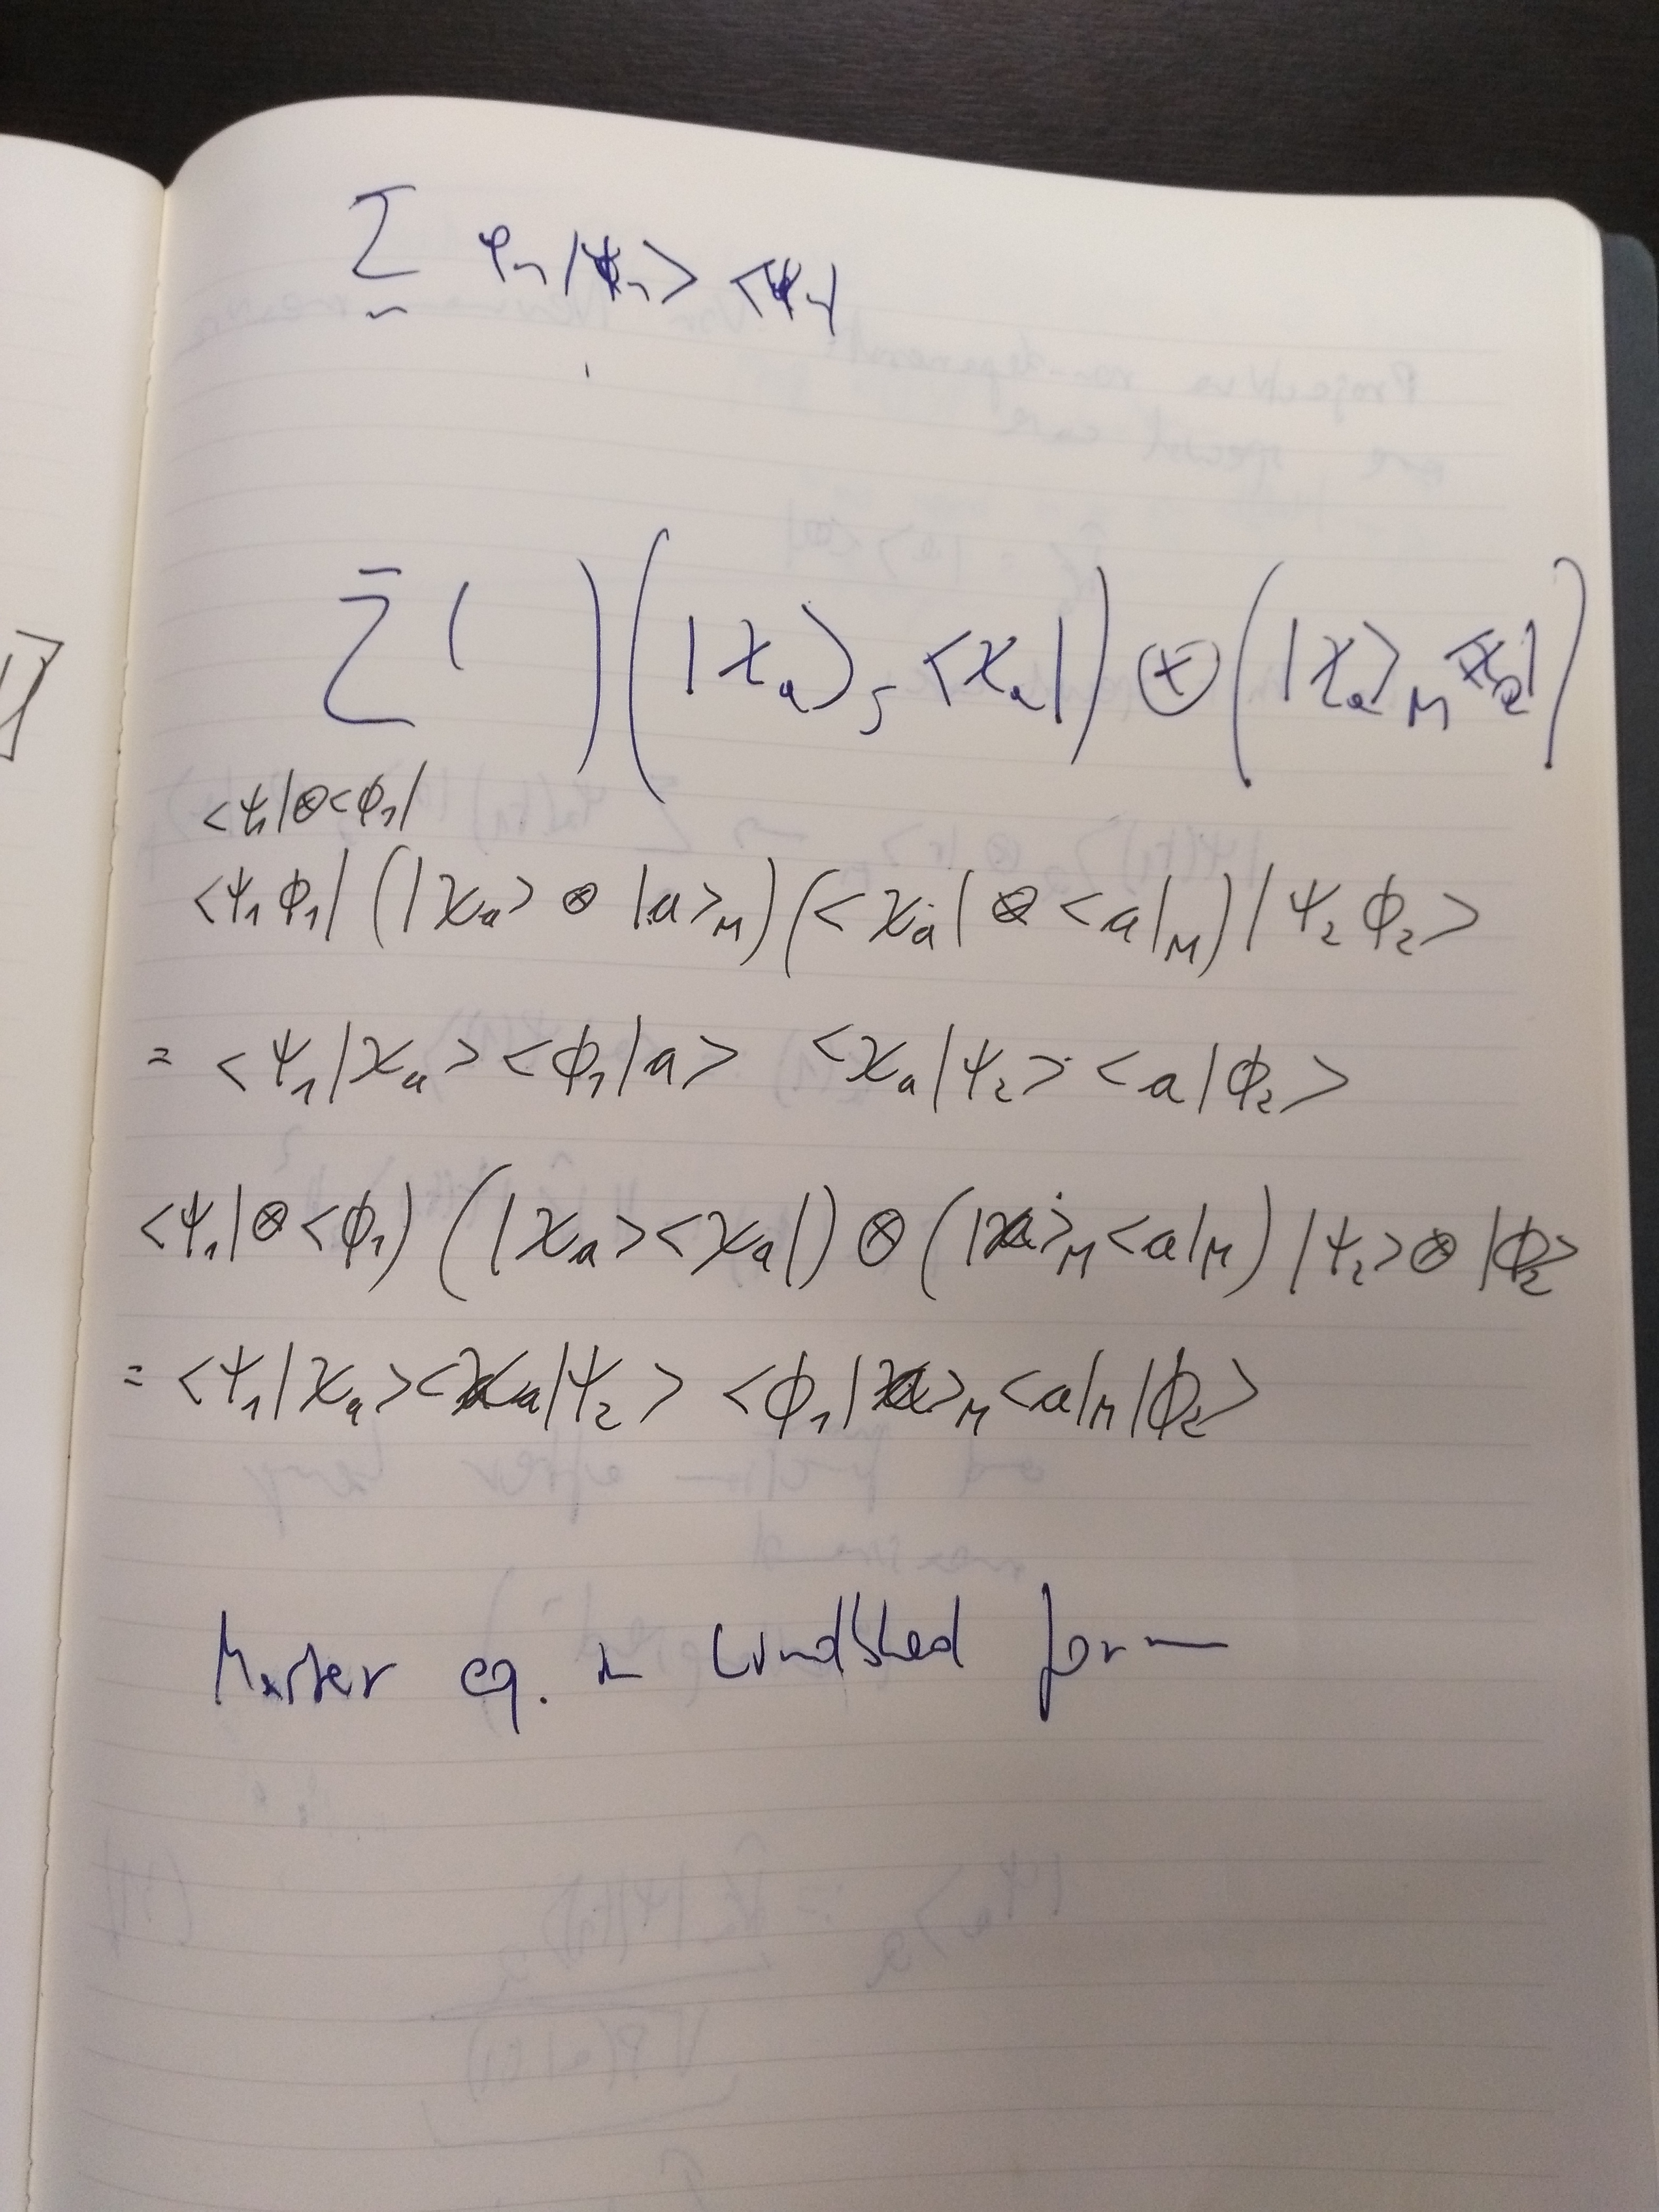
\includegraphics[width=\linewidth]{img/pw/qmem/4.jpg}
%\clearpage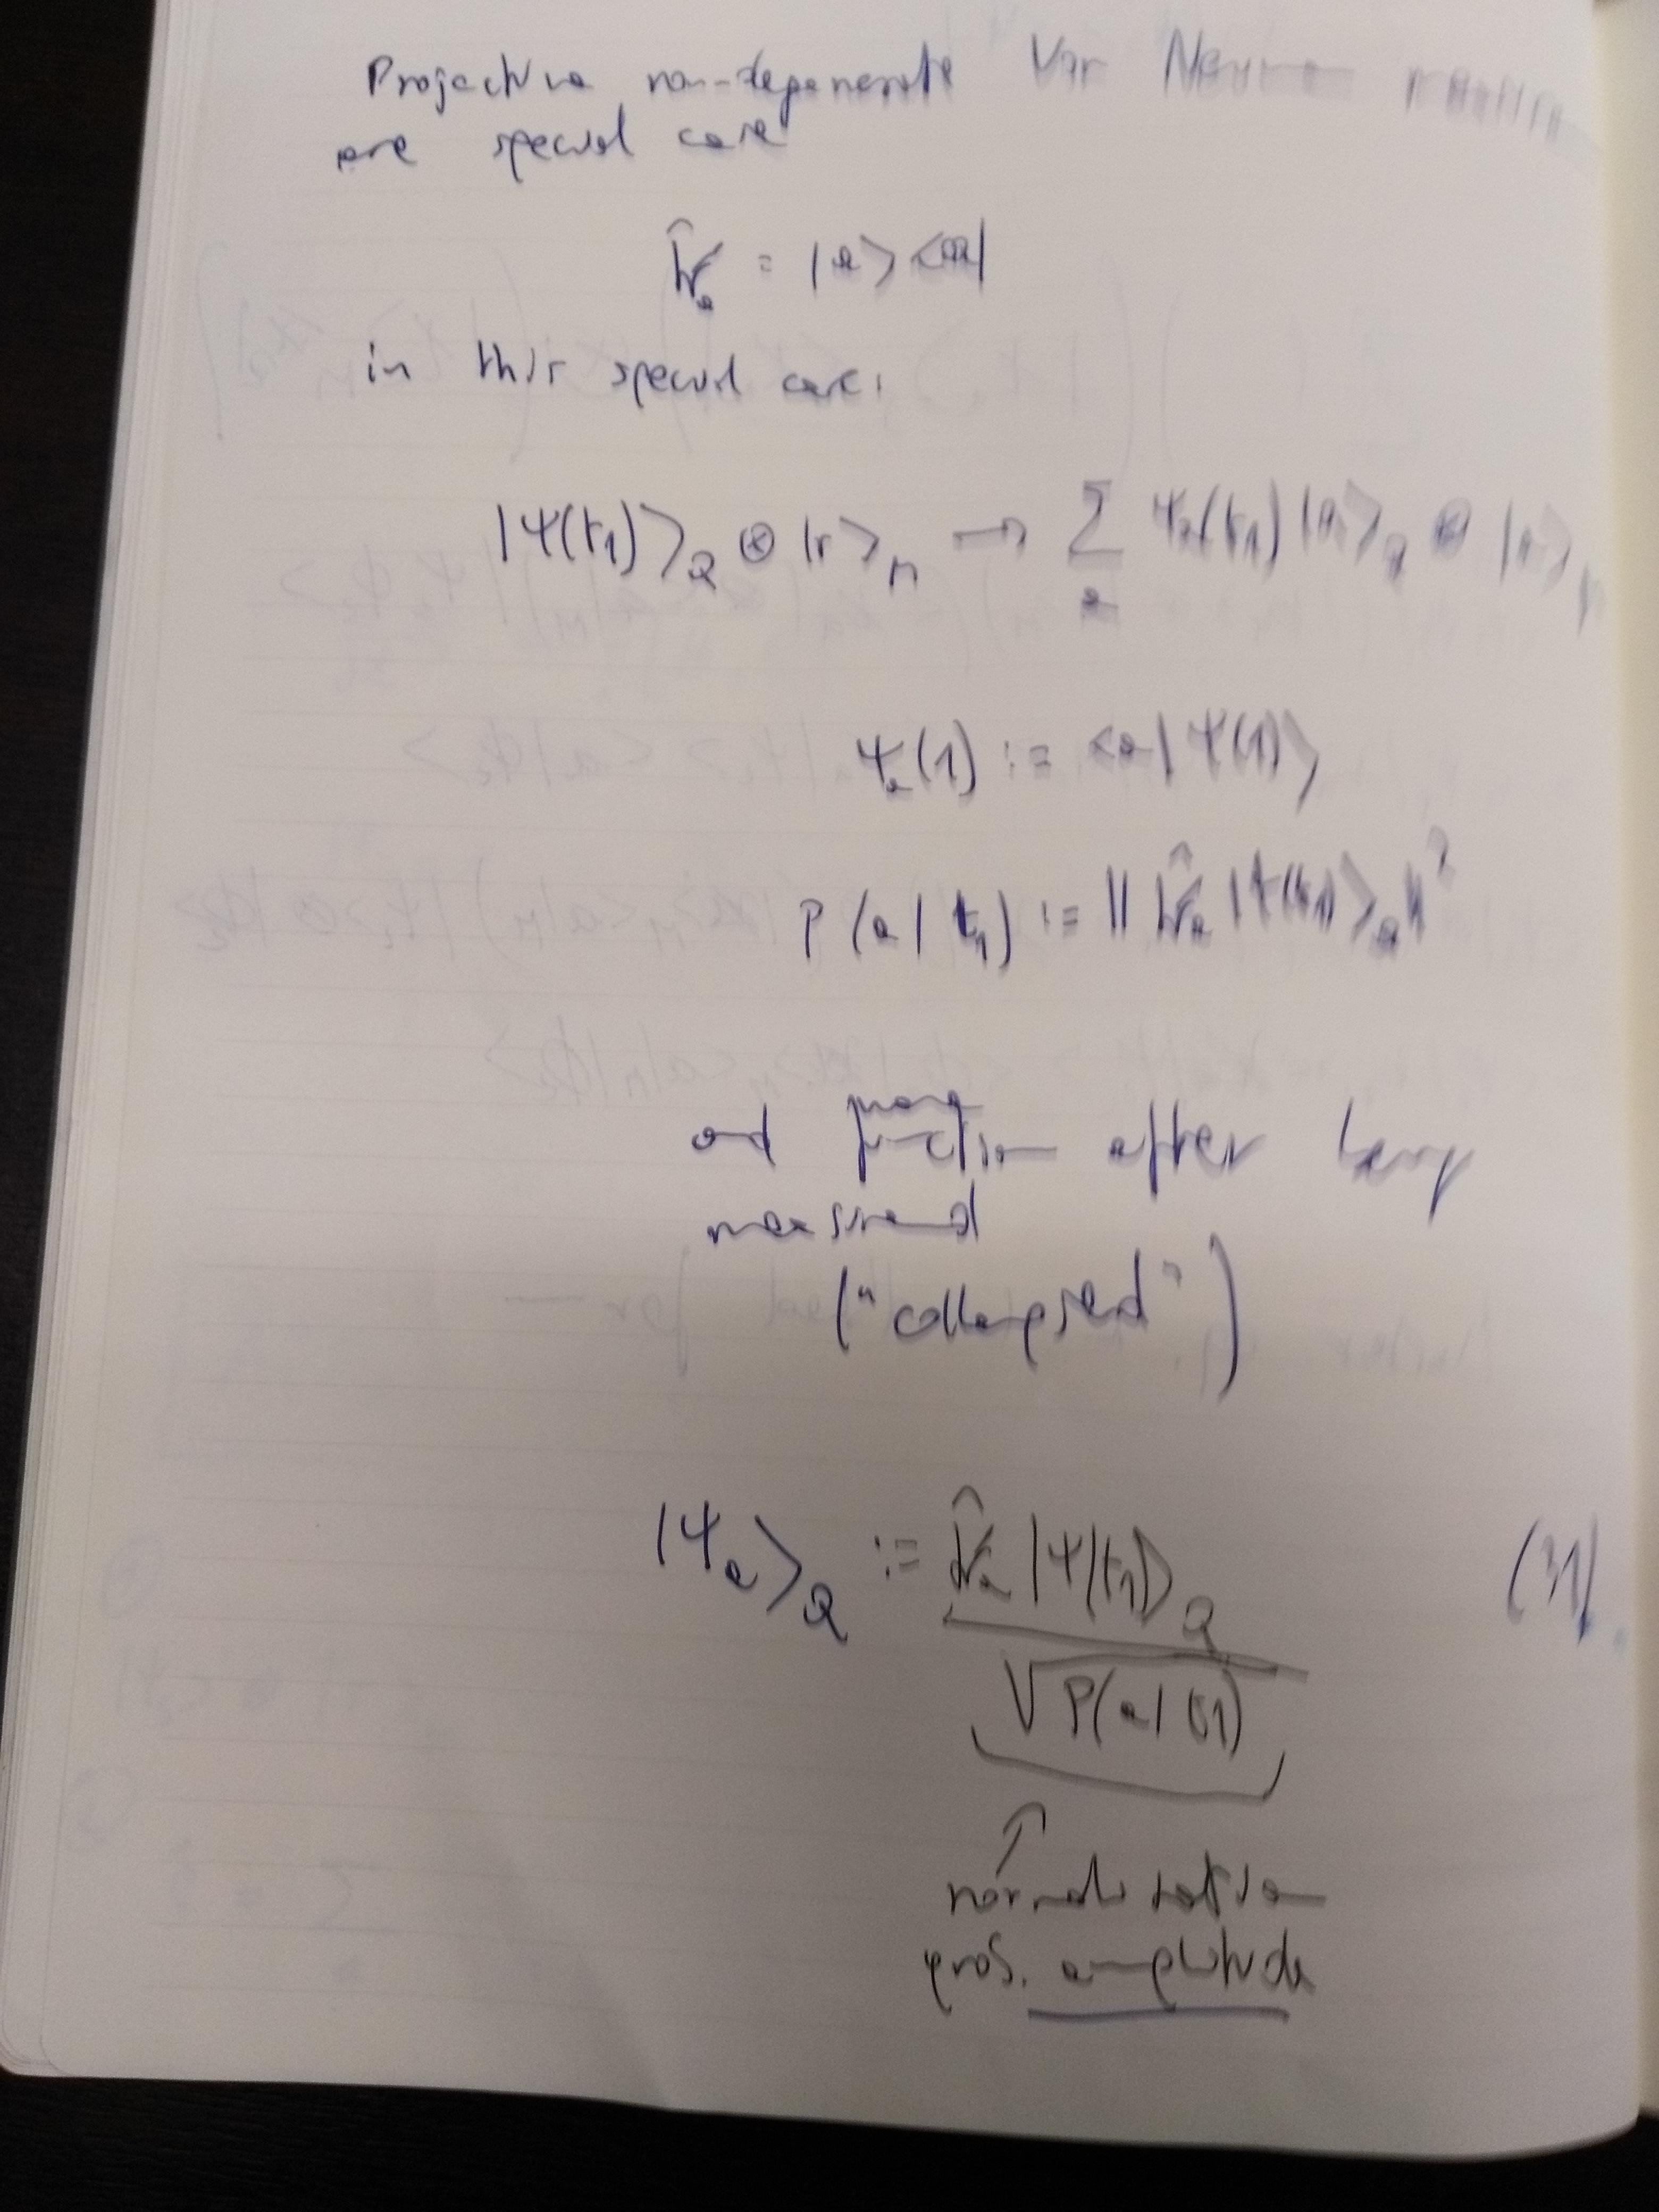
\includegraphics[width=\linewidth]{img/pw/qmem/5.jpg}

\section{Entanglement and decoherence}
See also \cite{EntanglementVsDecoherence}.

Decoherence is an irreversible process, it also happens in measurement.

According to Marletto and Vedral, arrow of time is increase in Entanglement
between the clock and the rest.

So, there seems to be a contradiction: is entanglement ``decreasing''
(i.e. destroyed by decoherence) with time
or increasing?

Perhaps we can avoid the contradiction saying that
entanglement between two finite systems is
destroyed while the entanglement of each of them with the universe
is increasing?

Or in other words, the entanglement of two clocks with the rest of universe
is increasing at the expenses of the entanglement between them?

And maybe we can conclude that two systems  of which we successfully
protect the entanglement from decoherence are not good clocks?

Or perhaps there's no relation\dots